In the first part we need to explain how the one-to-one alliance works and benefits the merchants.

\begin{figure}[H]
	\centering
	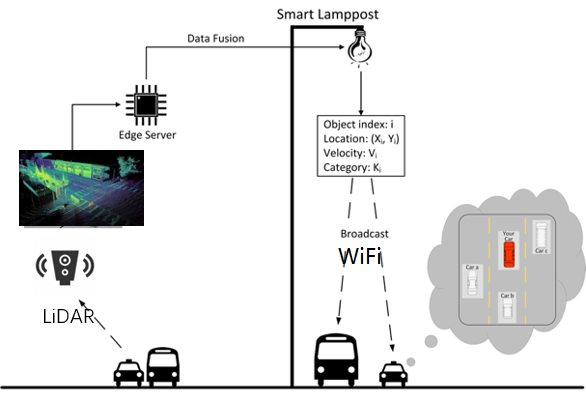
\includegraphics[width=\linewidth]{mechanism.png}
	\caption{the mechanism of the alliance}
	\label{fig:mechanism}
\end{figure}

Figure \ref{fig:mechanism} shows how the alliance system works. Suppose $x$ customers come to \A, do the purchase and obtain \RP{A}. Then they have needs for other products that \A\ does not offer. Since they can get a discount, a part of them will tend to go to \B. There they do the purchase, repeat the process and then return to \A. In the cycle, the number of the left customer is declining. As the customers return to the original merchant, the cycle comes to its end, which means the end of this round of benefit from \A\ to \B.